\documentclass{article}
\usepackage[utf8]{inputenc}
\usepackage[english]{babel}
\usepackage[table]{xcolor}
\usepackage{siunitx}
\usepackage{geometry}
\usepackage{graphicx}
\usepackage{longtable}
\usepackage{booktabs}
\usepackage{amsmath}
\usepackage{amssymb}
\usepackage{array}
\geometry{
  left=0.5in,
  top=0.2in,
  right=0.5in,
  bottom=0.5in
}
\sisetup{
  round-mode=places, % Rounds numbers
  round-precision=2, % to 2 places
}
\def\A#1{\textbf{#1}}
\def\B#1#2#3{\hspace*{#2}\textbf{#1}\hspace*{#3}}
\graphicspath{{./images/}} % image path
\title{Analysis of C. elegans on Drugs Lab Report}
\author{Philip Kim}
\date{\today}
\begin{document}
\maketitle
\vspace*{-1cm}
\begin{center}
  \begin{longtable}[c]{|c|r|r|r|}
    \toprule
    \textbf{\textcolor{white}{\#}} &
    \A{\textcolor{white}{Drug A -\ Control A}} &
    \A{\textcolor{white}{Drug A -\ Control A}} &
    \A{\textcolor{white}{Drug A -\ Control A}}\\
    \textbf{\#} &
    \B{Drug A}{0em}{3em} &
    \B{Control A}{0em}{2em} &
    \B{Drug A -\ Control A}{0em}{0em}\\
    \textbf{\textcolor{white}{\#}} &
    \textbf{\textcolor{white}{\#}} &
    \textbf{\textcolor{white}{\#}} &
    \textbf{\textcolor{white}{\#}}\\
    \midrule\endfirsthead%
    \toprule
    \textbf{\textcolor{white}{\#}} &
    \A{\textcolor{white}{Drug A -\ Control A}} &
    \A{\textcolor{white}{Drug A -\ Control A}} &
    \A{\textcolor{white}{Drug A -\ Control A}}\\
    \textbf{\#} &
    \B{Drug A}{0em}{3em} &
    \B{Control A}{0em}{2em} &
    \B{Drug A -\ Control A}{0em}{0em}\\
    \textbf{\textcolor{white}{\#}} &
    \textbf{\textcolor{white}{\#}} &
    \textbf{\textcolor{white}{\#}} &
    \textbf{\textcolor{white}{\#}}\\
    \midrule\endhead%
      1 & 40.20 & 22.40 & 17.80\\\midrule
      2 & 7.60 & 9.90 & -2.30\\\midrule
      3 & 0.00 & 6.20 & -6.20\\\midrule
      4 & 15.10 & 18.10 & -3.00\\\midrule
      5 & 10.50 & 20.50 & -10.00\\\midrule
      6 & 5.50 & 2.00 & 3.50\\\midrule
      7 & 22.50 & 25.00 & -2.50\\\midrule
      8 & 12.60 & 23.30 & -10.70\\\midrule
      9 & 3.00 & 15.00 & -12.00\\\midrule
      10 & 0.00 & 11.00 & -11.00\\
    \bottomrule
  \end{longtable}
  \begin{longtable}[c]{|c|r|r|r|}
    \toprule
    \textbf{\textcolor{white}{\#}} &
    \A{\textcolor{white}{Drug B -\ Control B}} &
    \A{\textcolor{white}{Drug B -\ Control B}} &
    \A{\textcolor{white}{Drug v -\ Control B}}\\
    \textbf{\#} &
    \B{Drug B}{0em}{3em} &
    \B{Control B}{0em}{2em} &
    \B{Drug B -\ Control B}{0em}{0em}\\
    \textbf{\textcolor{white}{\#}} &
    \textbf{\textcolor{white}{\#}} &
    \textbf{\textcolor{white}{\#}} &
    \textbf{\textcolor{white}{\#}}\\
    \midrule\endfirsthead%
    \toprule
    \textbf{\textcolor{white}{\#}} &
    \A{\textcolor{white}{Drug B -\ Control B}} &
    \A{\textcolor{white}{Drug B -\ Control B}} &
    \A{\textcolor{white}{Drug B -\ Control B}}\\
    \textbf{\#} &
    \B{Drug B}{0em}{3em} &
    \B{Control B}{0em}{2em} &
    \B{Drug B -\ Control B}{0em}{0em}\\
    \textbf{\textcolor{white}{\#}} &
    \textbf{\textcolor{white}{\#}} &
    \textbf{\textcolor{white}{\#}} &
    \textbf{\textcolor{white}{\#}}\\
    \midrule\endhead%
      1 & 33.70 & 26.30 & 7.40\\\midrule
      2 & 18.90 & 8.00 & 10.90\\\midrule
      3 & 15.00 & 9.00 & 6.00\\\midrule
      4 & 19.40 & 20.60 & -1.20\\\midrule
      5 & 41.20 & 13.57 & 27.63\\\midrule
      6 & 49.80 & 18.50 & 31.30\\\midrule
      7 & 36.10 & 21.90 & 14.20\\\midrule
      8 & 28.50 & 24.90 & 3.60\\\midrule
      9 & 23.90 & 22.10 & 1.80\\\midrule
      10 & 35.50 & 16.90 & 18.60\\
    \bottomrule
  \end{longtable}
  \begin{align*}
    n&= 10 \\
    \overline{x}&=\tfrac{x_1 + x_2 + \cdots + x_n}{n}\\
    \sigma_x&= \sqrt{\tfrac{\left|x_1 - \overline{x}\right|^2 + \cdots + \left|x_n - \overline{x}\right|^2}{n - 1}}\\
    \epsilon_x&= 2\times\left(\tfrac{\sigma_x}{\sqrt{n}}\right)
  \end{align*}
  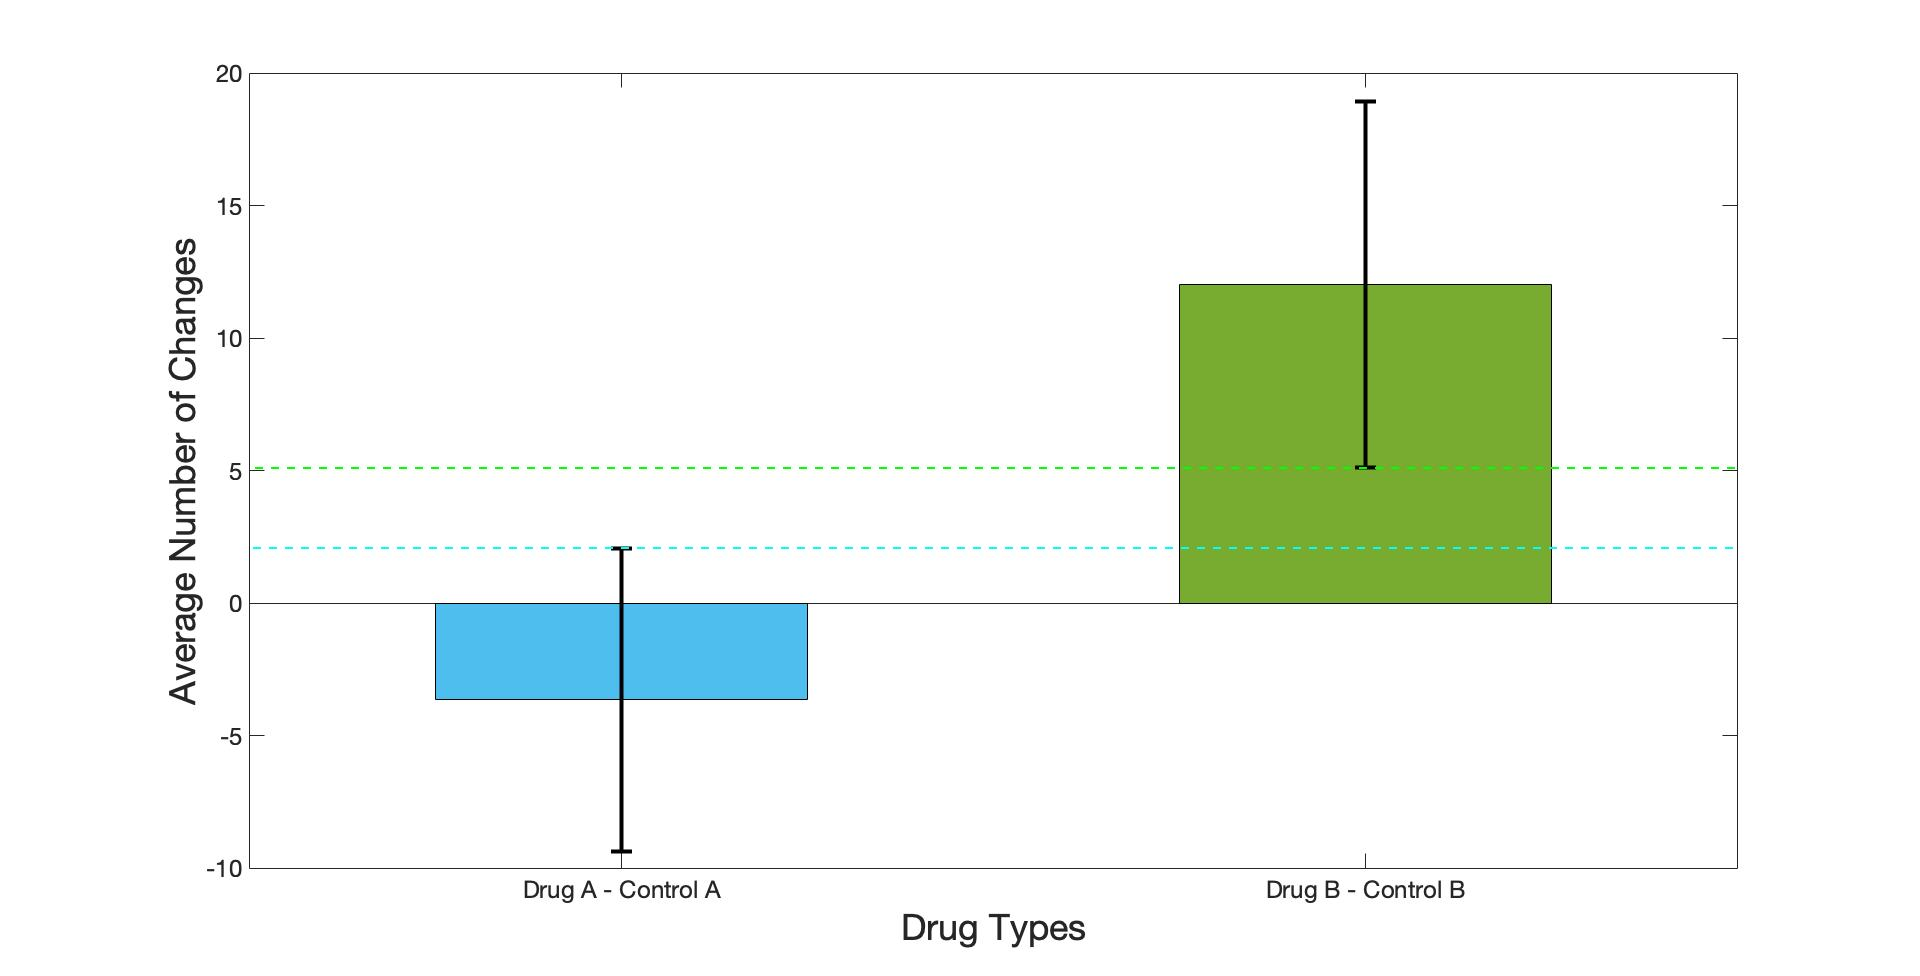
\includegraphics[width=\textwidth]{graph.jpg}
  \fbox{\begin{minipage}{53em}
    \begin{enumerate}
      \item What was your hypothesis?
      \item[] a
      \item Does the data support your hypothesis? In other words, what were the results of the experiment? Did Drug A have a significant positive or negative effect? Did Drug B have a significant positive or negative effect? (Significance = the confidence intervals do not extend past 0)
      \item[] b
      \item If the data does not show significance, why might this be?
      \item[] c
      \item (In reference to experiment video) Do you think it's an issue that Robyn knew which side of the slide was the control and which side contained the drug? Could this influence results?
      \item[] d
    \end{enumerate}
  \end{minipage}}
\end{center}
\end{document}